\documentclass{beamer}
\usepackage{amssymb,latexsym,amssymb,amsmath,amsbsy,amsopn,amstext,upgreek}
\usepackage{color,multicol}
\usepackage{graphicx,wrapfig,fancybox,watermark,picins,graphics}
\usepackage{pgf}
\usepackage{movie15}
\usepackage{hyperref}
\usepackage{pdfpages}
\usepackage{listings}
\lstset{language=Matlab}
\hypersetup{
    pdfpagemode=FullScreen, % show in full screen?
}
\usepackage{algorithm}
\usepackage{algorithmic}
\renewcommand{\algorithmicrequire}{\textbf{Input:}}
\renewcommand{\algorithmicensure}{\textbf{Output:}}
% reference entry
\usepackage{bibentry, natbib}
% reference style
\bibliographystyle{IEEEtran} 
%reference lib
\nobibliography{refs}

\usepackage[red,numbers]{beamerthemeHongKong}
\usefonttheme[professionalfonts]{serif}

\title[Tutorial 9]{Tutorial 9: The Assignment 4}
\author[COMP210]{Qu Xiaofeng\texorpdfstring{, Teaching Asistant}{}}
\institute{COMP210\\Discrete Structure}
\date{\today}

\begin{document}

\frame{\titlepage}

\section*{Table of Contents}
    \begin{frame}{\secname}
        \tableofcontents
    \end{frame}

\AtBeginSubsection[] {
    \begin{frame}<handout:0>{Outline}
        \tableofcontents[current,currentsubsection]
    \end{frame}
}
\section[Review]{Review of Algorithm \& Counting methods}
    \begin{frame}[c,shrink]{\secname}
        \label{}
        \centerline{\includegraphics[height=0.85\textheight,page=2]{algo_counting}}
    \end{frame}
    \begin{frame}[c,shrink]{\secname\ cont.}
        \centerline{\includegraphics[height=0.85\textheight,page=3]{algo_counting}}
    \end{frame}
    \begin{frame}[c,shrink]{\secname\ cont.}
        \centerline{\includegraphics[height=0.85\textheight,page=4]{algo_counting}}
    \end{frame}
    \begin{frame}[c,shrink]{\secname\ cont.}
        \centerline{\includegraphics[height=0.85\textheight,page=5]{algo_counting}}
    \end{frame}
    \begin{frame}[c,shrink]{\secname\ cont.}
        \centerline{\includegraphics[height=0.85\textheight,page=6]{algo_counting}}
    \end{frame}
    
    
    
\section{Problems}



    \subsection{Problem 1}
    
        \begin{frame}[c]{\subsecname}
            \textit{Write an algorithm that reverses a string $s_1,\ldots,s_n$.\\
            Example: If the sequence is AMY BRUNO ELIE,\\
            the reversed sequence is ELIE BRUNO AMY.}            
        \end{frame}
        
        \begin{frame}[c,shrink]{\subsecname\ cont.}          
            \begin{algorithm}[H]
                \caption {Reverse string s}
                \label{alg1}
                \begin{algorithmic}[1]
                    \REQUIRE String s, where s ends with EOL
                    \STATE $i \leftarrow 1$, $word\_cnt \leftarrow 0$ \COMMENT{Parsing}
                    \WHILE{$s(i) \neq EOL$}
                    \WHILE{$s(i)=''\!\textvisiblespace\ ''$}
                    \STATE $i \leftarrow i+1$
                    \ENDWHILE
                    \IF{$s(i) \neq EOL$}
                    \STATE $word\_cnt \leftarrow word\_cnt+1$, $char\_cnt \leftarrow 1$
                    \WHILE{$s(i) \neq EOL$ \AND $s(i)=''\!\textvisiblespace\ ''$}
                    \STATE $word[word\_cnt][char\_cnt] \leftarrow s(i)$
                    \STATE $char\_cnt \leftarrow char\_cnt + 1$, $i \leftarrow i+1$
                    \ENDWHILE
                    \ENDIF
                    \ENDWHILE
                    \FOR[Output]{$i \leftarrow word\_cnt$ \TO $1$}
                    \PRINT $word[i]$
                    \ENDFOR \qed
                \end{algorithmic}
            \end{algorithm}        
        \end{frame}
        
        
        
    \subsection{Problem 4}
    
        \begin{frame}[c,shrink]{Common Growth Functions}
            \begin{table}[tp]%
                \caption{Common Growth Functions\ (Table 4.3.3)}
                \label{cgf}\centering%
                \begin{tabular}{ll}
                    \hline%\toprule%
                    Theta Form             & Name         \\\hline%\otoprule%
                    $\Theta(1)         $   & Constant     \\
                    $\Theta(\lg\lg{n}) $   & Log log      \\
                    $\Theta(\lg{n})    $   & Log          \\
                    $\Theta(n)         $   & Linear       \\
                    $\Theta(n\lg{n})   $   & n log n      \\
                    $\Theta(n_2)       $   & Quadratic    \\
                    $\Theta(n_3)       $   & Cubic        \\
                    $\Theta(n_k)       $   & Polynomial   \\
                    $\Theta(c_n)       $   & Exponential  \\
                    $\Theta(n!)        $   & Factorial    \\\hline%\bottomrule
                \end{tabular}
            \end{table}
        \end{frame}
        
        \begin{frame}[c,shrink]{\subsecname{}.1}
            \textit{Select a theta notation from Table 4.3.3 for $3n^2+2n\lg{n}$.}\pause     
            \begin{align*}
                0 < \lg{n}		&\leq n 	\hfill &for\ all\ n \geq 1\\
                0 < 2n\lg{n} 	&\leq 2n^2 \hfill &for\ all\ n \geq 1
            \end{align*}\pause
            Then the dominating term is\ $3n^2$.\\ \pause
            \begin{overprint}
            \onslide<4|handout:0>
            \begin{align*}
            f(n)&= 3n^2+2n\lg{n} > 3n^2=C_1n^2,\ where\ C_1=3\\
            f(n)&=\Omega(n^2)
            \end{align*}
            \onslide<5|handout:0>   
            \begin{align*}
            f(n)&= 3n^2+2n\lg{n} > 3n^2=C_1n^2,\ where\ C_1=3\\
            f(n)&=\Omega(n^2)\\
            f(n)&= 3n^2+2n\lg{n} \leq 3n^2+2n^2=C_2n^2,\ where\ C_2=5\\
            f(n)&=O(n^2)
            \end{align*}
            \onslide<6->   
            \begin{align*}
            f(n)	&= 3n^2+2n\lg{n} > 3n^2=C_1n^2,\ where\ C_1=3\\
            f(n)	&= \Omega(n^2)\\
            f(n)	&= 3n^2+2n\lg{n} \leq 3n^2+2n^2=C_2n^2,\ where\ C_2=5\\
            f(n)	&= O(n^2)\\
            f(n)	&= \Theta(n^2)  \qed
            \end{align*}
            \end{overprint}
        \end{frame}
        
        \begin{frame}[c,shrink]{\subsecname{}.3}
            \textit{Select a theta notation from Table 4.3.3 for $\frac{(n+1)(n+3)}{n+1}$}\\
            $\;$\\\pause  
            For all $n > -1$, the equation could be simplified as bellow,   
            \begin{align*}
                \frac{(n+1)(n+3)}{n+1}			&= n+3\ 
            \end{align*}\pause
            So for all $n \geq 3$,
            \begin{align*}
                f(n) = \frac{(n+1)(n+3)}{n+1} &\geq n = C_1n = \Omega(n)\\
                                         f(n) &\leq 2n = C_2n = O(n)
            \end{align*} \pause
            Then           
            \begin{align*}
                f(n) = \frac{(n+1)(n+3)}{n+1} &= \Theta(n) \qed
            \end{align*}
        \end{frame}
        
        
        
    \subsection{Problem 5.1}
    
        \begin{frame}[c,containsverbatim]{\subsecname}
            \textit{Express in theta notation the number of times the statement x = x + 1 is
executed.}
            \begin{lstlisting}
for i = 1 to n
    for j = 1 to n
        x = x + 1;
            \end{lstlisting}
        \end{frame}
        
        \begin{frame}[c]{\subsecname\ cont.}
            The basic operation runs 1 times. The for loops of j, runs n times, and the outer for loops of i runs n times. So based on the multiplication principle. Then total number is $1\times n \times n=n^2$.\pause
            \begin{align*}
            f(n)=n^2=\Theta(n^2) \qed
            \end{align*}
        \end{frame}
        
        
        
    \subsection{Problem 6}
    
        \begin{frame}[c,shrink]{\subsecname}
            \textit{show that $\lg(n^k+c) = \Theta(\lg{n})$ for every fixed $k>0$ and $c>0$.}
            \begin{overprint}
            \onslide<2|handout:0>
            \begin{align*}
                for\ all\ n \geq c^{\frac{1}{k}},
            \end{align*}
            \onslide<3|handout:0>
            \begin{align*}
                for\ all\ n \geq c^{\frac{1}{k}},&\\
                \lg{(n^k+c)} &\leq \lg(2n^k)\\
                		  &=    k\lg{n}+\lg{2}\\
                		  &\leq C_1\lg{n},\ where\ C_1= k+1,\ n\geq 2\\
                		  &=    O(\lg{n})
            \end{align*}
            \onslide<4|handout:0>
            \begin{align*}
                for\ all\ n \geq c^{\frac{1}{k}},&\\
                \lg{(n^k+c)} &\leq \lg(2n^k)\\
                		  &=    k\lg{n}+\lg{2}\\
                		  &\leq C_1\lg{n},\ where\ C_1= k+1,\ n\geq 2\\
                		  &=    O(\lg{n})\\
                \lg{(n^k+c)} &\geq \lg(n^k) = k\lg{n}\\
                		  &= C_2\lg{n},\ where\ C_2= k\\
                		  &= \Omega(\lg{n})
            \end{align*}
            \onslide<5>
            \begin{align*}
                for\ all\ n \geq c^{\frac{1}{k}},&\\
                \lg{(n^k+c)} &\leq \lg(2n^k)\\
                		  &=    k\lg{n}+\lg{2}\\
                		  &\leq C_1\lg{n},\ where\ C_1= k+1,\ n\geq 2\\
                		  &=    O(\lg{n})\\
                \lg{(n^k+c)} &\geq \lg(n^k) = k\lg{n}\\
                		  &= C_2\lg{n},\ where\ C_2= k\\
                		  &= \Omega(\lg{n})\\
                \lg{(n^k+c)} &= \Theta(\lg{n}) \qed
            \end{align*}
            \end{overprint}
        \end{frame}
        

        
\section{Problems cont.}

                
        
    \subsection{Problem 10}
    
        \begin{frame}[c,shrink]{\subsecname}
            \textit{Two dice are rolled, one blue and one red. How many outcomes give the sum of
2 or the sum 12?}
            \begin{overprint}
            \onslide<2|handout:0>
            \begin{table}[tp]%
                \caption{Outcomes of dice}
                \label{dicetable1}\centering%
                \begin{tabular}{ccc}
                    \hline%\toprule%
                      Sum 	& Blue  & Red 	\\\hline%\otoprule%
                     2 	& 1	   & 1 	\\\hline%\bottomrule
                \end{tabular}
            \end{table}
            \onslide<3|handout:0>
            \begin{table}[tp]%
                \caption{Outcomes of dice}
                \label{dicetable2}\centering%
                \begin{tabular}{ccc}
                    \hline%\toprule%
                      Sum 	& Blue  & Red 	\\\hline%\otoprule%
                     2 	& 1	   & 1 	\\\hline
                     12 	& 6	   & 6 	\\\hline%\bottomrule
                \end{tabular}
            \end{table}
            \onslide<4->
            \begin{table}[tp]%
                \caption{Outcomes of dice}
                \label{dicetable3}\centering%
                \begin{tabular}{ccc}
                    \hline%\toprule%
                      Sum 	& Blue  & Red 	\\\hline%\otoprule%
                     2 	& 1	   & 1 	\\\hline
                     12 	& 6	   & 6 	\\\hline
                     8 	& 2	   & 6 	\\
                      	& 3	   & 5 	\\
                      	& 4	   & 4 	\\
                      	& 5	   & 3 	\\
                      	& 6	   & 2 	\\\hline%\bottomrule
                \end{tabular}
            \end{table}
            \end{overprint}
            \onslide<5>{1 outcome gives the sum of 2;\\
            1 outcome gives the sum of 12.\qed}
        \end{frame}
        
        
        
    \subsection{Problem 12.2}
    
        \begin{frame}[c]{\subsecname}
            \textit{For integers from 5 to 200, inclusive. How many do not contain the digit 0?}\\
            $\;$\\
            \begin{overprint}
            \onslide<2|handout:0>
                \begin{tabular}{lcr}
                     Single digit		& 5,6,7,8,9 	& 5 	
                \end{tabular}            
            \onslide<3|handout:0>
                \begin{tabular}{lcr}
                     Single digit		& 5,6,7,8,9 	& 5 	\\
                     Two digit  (xx) 		& 9$\times$9 	& 81 	
                \end{tabular}   
            \onslide<4->
                \begin{tabular}{lcr}
                     Single digit		& 5,6,7,8,9 	& 5 	\\
                     Two digit (xx)  		& 9$\times$9 	& 81 	\\
                     Three digit (1xx)  	& 9$\times$9 	& 81 	
                \end{tabular}   
            \end{overprint}
            $\;$\\
            \onslide<5>{By Addition principle, the total is 167. \qed}
        \end{frame}
        
        
        
    \subsection{Problem 14.1}
    
        \begin{frame}[c,shrink]{\subsecname}
            \textit{How many symmetric and antisymmetric relations are there on an n-element
set?}\\\pause
                \begin{definition}
			    A relation R on a set X is \alert{symmetric} if $\forall$ x,y $\in$ X, if (x,y) $\in$ R, then (y,x) $\in$ R.\{Definition 3.3.9\}
                \end{definition}\pause
                \begin{definition}
			    A relation R on a set X is \alert{antisymmetric} if $\forall$ x,y $\in$ X, if (x,y) $\in$ R and (y,x) $\in$ R then x=y. \{Definition 3.3.12\}
                \end{definition}
        \end{frame}
    
        \begin{frame}[c]{\subsecname\ cont.}
            Symmetric and antisymmetric means \alert{no pairwise relation}\\$\;$\\\pause
            e.g. xRy doesn't exist if x $\neq$ y\\$\;$\\\pause
            For each element, two ways: self loop or not.\\$\;$\\\pause
            $\Rightarrow$ 2$\times$2$\times\cdots\times$2 by Multiplication principle\\$\;$\\\pause
            So, there are $2^n$ summetric and antisymmetric relations on an n-element set.\qed
        \end{frame}
        
        
        
\subsection{Some Typo Errors}

    \begin{frame}[c,shrink]{\subsecname}
        \begin{itemize}
        \item
Problem 2: should be Page \alert{185} ; ... receives \alert{as} input ...
        \item
Problem 5: should be ... notation \alert{for} the number ...
        \item
Problme 7: the equation should be \[\alert{\sum^k_{i=0}}\lg(\frac{n}{2^i})=\Theta(\lg^2n)\]
        \item
Problme 8: there are \alert{two} problem 8s. Please mark \alert{the second problem 8} as \alert{problem 8.4}, for we can take the following numbers as they are now.
        \item
Problme 8.2: the equation shoul be \[...\ +\alert{\frac{1}{n-1}}.\]
        \item
Problme 12.4: shoul be $...\ \alert{y>z}.$ \qed
        \end{itemize}
    \end{frame}
        
        
        
\section*{Q \& A}

    \begin{frame}<handout:0>[c]{\secname}
        \centerline{\Huge{Questions about the problems?}}
    \end{frame}
    
    
    
\end{document}



